Für die Organisation wurde das Projektmanagement Tool \textbf{Basecamp} verwendet.

“Basecamp ist die Projektmanagementplattform, die kleinen Teams hilft, schneller voranzukommen und größere Fortschritte zu erzielen , als sie es jemals für möglich gehalten hätten.”
\newline
(vgl. \url{https://basecamp.com/}; Zugriff: 17.03.2024)

Basecamp wurde bereits in dem Unternehmen als Kommunikations- und Projektverwaltungsprogramm verwendet. Hierbei wurde ein neues Projekt für die Diplomarbeit erstellt, zu welchem alle Mitarbeiter:innen hinzugefügt wurden, die dabei mit uns in Verbindung stehen.
Kommunikation und Organisation fand dabei ausschließlich in diesem Basecamp-Projekt statt. Das erleichterte den Prozessverlauf, da sich alles relevante an einem gesammelten Ort befand und man dadurch ständig eine Übersicht hatte und Entscheidungen nachvollziehen konnte.
Ein Projekt in Basecamp hat immer den selben Aufbau:

\begin{figure}[h!]
    \centering
    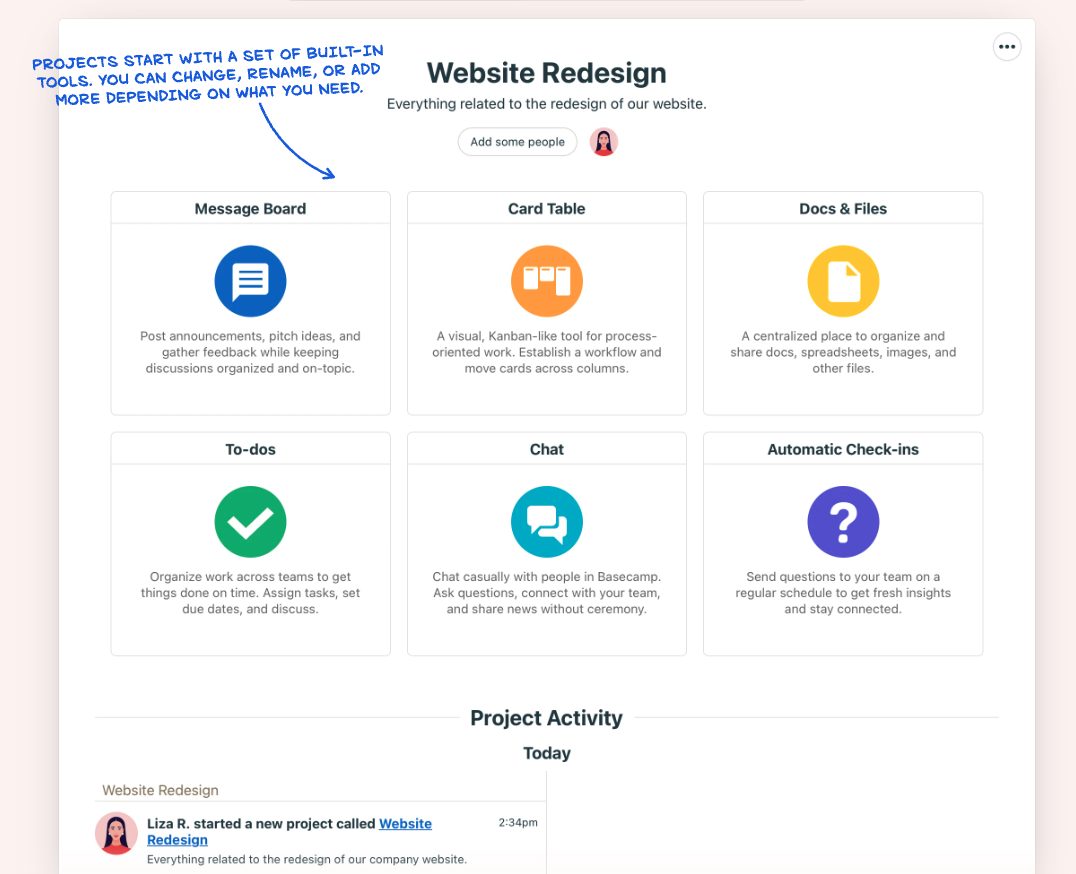
\includegraphics[width=0.8\textwidth]{pics/basecamp-project-overview.png}
    \caption{Basecamp Projekt}
    \cite{basecamp_project}
    \label{fig:mesh1}
\end{figure}

Es gibt ein sogenanntes Message Board, in welchen Ankündigungen oder ähnliche wichtige Nachrichten gespeichert werden können. Des weiteren gibt es einen Card Table, welcher ein Kanban Board beinhaltet, welches einen agilen Projektverlauf unterstützt. Dokumente oder wichtige Datein können im Unterpunkt Docs und Files abgespeichert werden. Für To-dos oder auch für den allgemeinen Chat gibt es ebenfalls Unterseiten. Und zuletzt gibt es die Möglichkeit automatische Check-ins zu machen um aktiv mit den anderen Teammitgliedern vernetzt und am laufenden Stand zu sein.

Wir haben dabei hauptsächlich die To-dos und die Chat-Funktion verwendet. Erwähnenswert ist auch, dass die Kommunikation ausschließlich über Basecamp stattgefunden hat und die Arbeit damit im Allgemeinen gut funktioniert hat.